%%%%%%%%%%%%%%%%%%%%%%%%%%%%%%%%%%%%%%%%%
% Beamer Presentation
% LaTeX Template
% Version 1.0 (10/11/12)
%
% This template has been downloaded from:
% http://www.LaTeXTemplates.com
%
% License:
% CC BY-NC-SA 3.0 (http://creativecommons.org/licenses/by-nc-sa/3.0/)
%
%%%%%%%%%%%%%%%%%%%%%%%%%%%%%%%%%%%%%%%%%

%----------------------------------------------------------------------------------------
%	PACKAGES AND THEMES
%----------------------------------------------------------------------------------------

\documentclass[UTF8]{ctexbeamer}

\usepackage{hyperref}
\hypersetup{
  colorlinks=true,
  linkcolor=red,
  anchorcolor=blue,
  citecolor=green
}

\mode<presentation> {

% The Beamer class comes with a number of default slide themes
% which change the colors and layouts of slides. Below this is a list
% of all the themes, uncomment each in turn to see what they look like.

%\usetheme{default}
%\usetheme{AnnArbor}
%\usetheme{Antibes}
%\usetheme{Bergen}
%\usetheme{Berkeley}
%\usetheme{Berlin}
%\usetheme{Boadilla}
%\usetheme{CambridgeUS}
%\usetheme{Copenhagen}
%\usetheme{Darmstadt}
%\usetheme{Dresden}
%\usetheme{Frankfurt}
%\usetheme{Goettingen}
%\usetheme{Hannover}
%\usetheme{Ilmenau}
%\usetheme{JuanLesPins}
%\usetheme{Luebeck}
\usetheme{Madrid}
%\usetheme{Malmoe}
%\usetheme{Marburg}
%\usetheme{Montpellier}
%\usetheme{PaloAlto}
%\usetheme{Pittsburgh}
%\usetheme{Rochester}
%\usetheme{Singapore}
%\usetheme{Szeged}
%\usetheme{Warsaw}

% As well as themes, the Beamer class has a number of color themes
% for any slide theme. Uncomment each of these in turn to see how it
% changes the colors of your current slide theme.

%\usecolortheme{albatross}
%\usecolortheme{beaver}
%\usecolortheme{beetle}
%\usecolortheme{crane}
%\usecolortheme{dolphin}
%\usecolortheme{dove}
%\usecolortheme{fly}
%\usecolortheme{lily}
%\usecolortheme{orchid}
%\usecolortheme{rose}
%\usecolortheme{seagull}
%\usecolortheme{seahorse}
%\usecolortheme{whale}
%\usecolortheme{wolverine}

%\setbeamertemplate{footline} % To remove the footer line in all slides uncomment this line
%\setbeamertemplate{footline}[page number] % To replace the footer line in all slides with a simple slide count uncomment this line

%\setbeamertemplate{navigation symbols}{} % To remove the navigation symbols from the bottom of all slides uncomment this line
}

\usepackage{graphicx} % Allows including images
\graphicspath{{./figs/}}
\usepackage{booktabs} % Allows the use of \toprule, \midrule and \bottomrule in tables
\usepackage{longtable}
% Fonts
% \usepackage{libertine}
% \setmonofont{Courier}
\setCJKsansfont[ItalicFont=Noto Serif CJK SC Black, BoldFont=Noto Sans CJK SC Black]{Noto Sans CJK SC}

%----------------------------------------------------------------------------------------
%	TITLE PAGE
%----------------------------------------------------------------------------------------

\title[第1讲]{第2讲 :操作系统与系统结构和程序设计语言} % The short title appears at the bottom of every slide, the full title is only on the title page

\author{向勇、陈渝} % Your name
\institute[清华大学] % Your institution as it will appear on the bottom of every slide, may be shorthand to save space
{
清华大学计算机系 \\ % Your institution for the title page
\medskip
\textit{xyong,yuchen@tsinghua.edu.cn} % Your email address
}
\date{\today} % Date, can be changed to a custom date

\begin{document}

\begin{frame}
\titlepage % Print the title page as the first slide
\end{frame}

\begin{frame}
\frametitle{提纲} % Table of contents slide, comment this block out to remove it
\tableofcontents % Throughout your presentation, if you choose to use \section{} and \subsection{} commands, these will automatically be printed on this slide as an overview of your presentation
\end{frame}

%----------------------------------------------------------------------------------------
%	PRESENTATION SLIDES
%----------------------------------------------------------------------------------------

%------------------------------------------------
\section{第一节:RISC-V -- 从OS角度 } % Sections can be created in order to organize your presentation into discrete blocks, all sections and subsections are automatically printed in the table of contents as an overview of the talk
%------------------------------------------------

\subsection{Why RISC-V} % A subsection can be created just before a set of slides with a common theme to further break down your presentation into chunks
\subsection{RISC-V特权架构}

\begin{frame}
	
	\frametitle{Why RISC-V}
	
	\begin{figure}
		\centering
		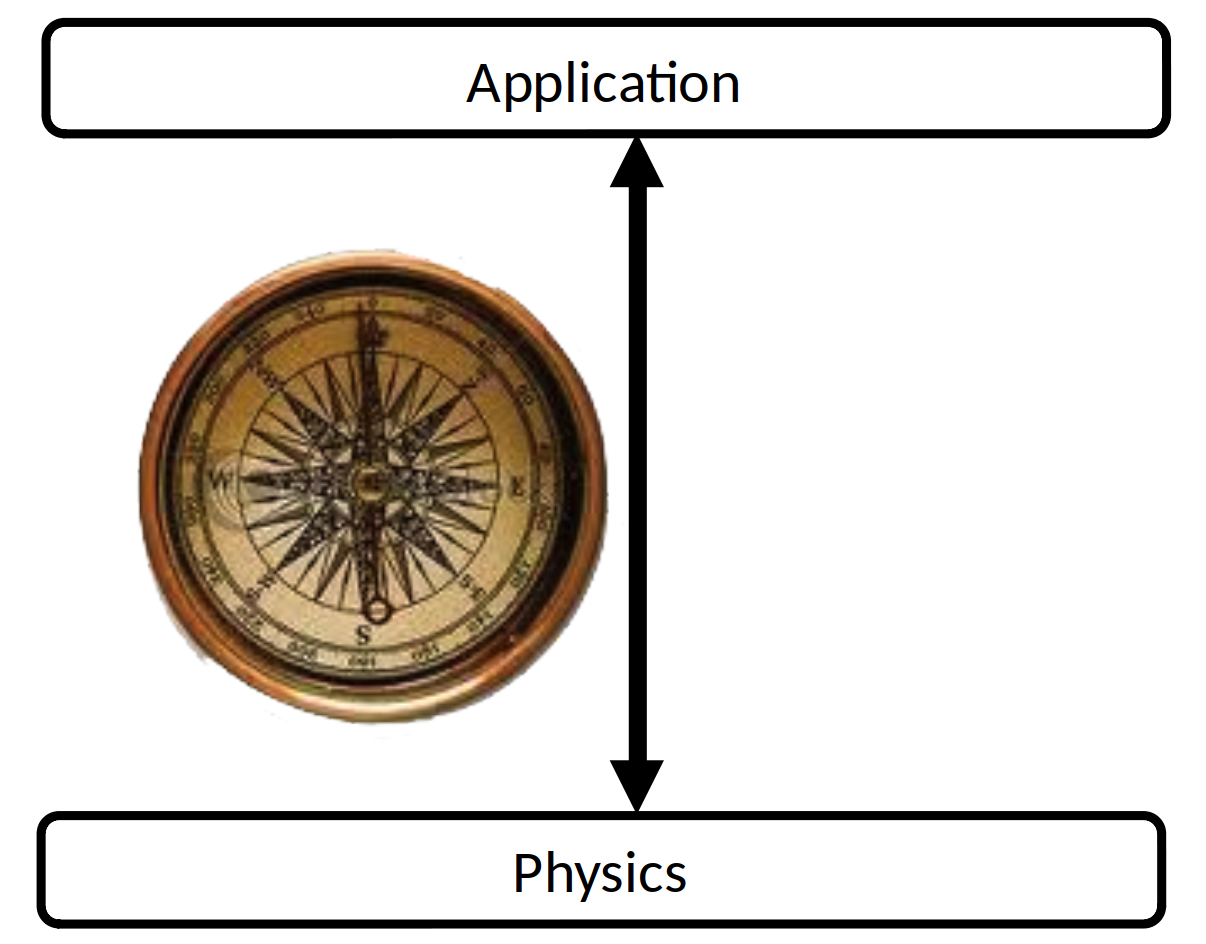
\includegraphics[width=0.45\linewidth]{computer-arch-app}
		\caption{计算机系统$_{[CS-152 Berkeley]}$}
	\end{figure}
	
	广义的定义, 计算机系统(computer architecture)是一种抽象层次的设计,用于实现可有效使用现有制造技术的信息处理应用。$_{[CS-152 Berkeley]}$
\end{frame}


\begin{frame}
	
	\frametitle{Why RISC-V}
	
	\begin{figure}
		\centering
		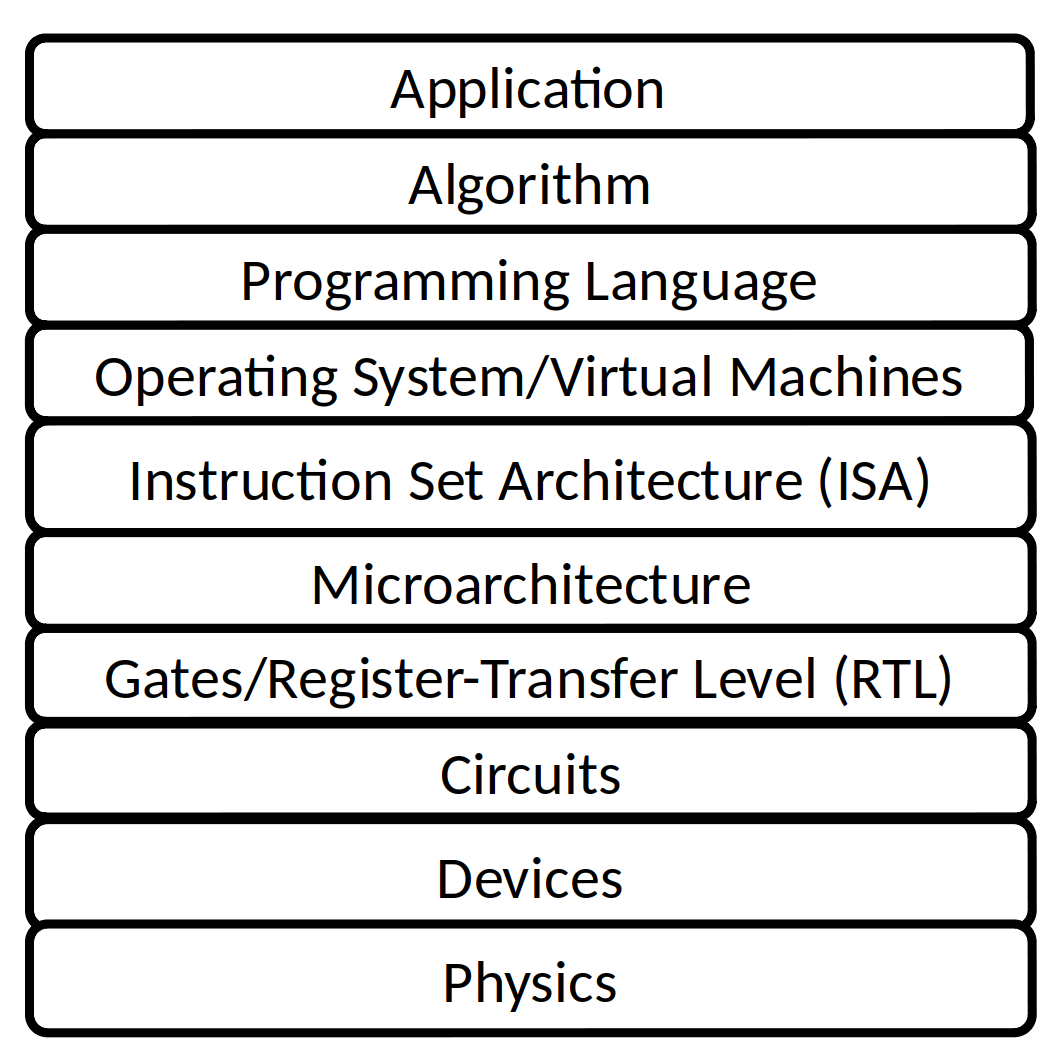
\includegraphics[width=0.45\linewidth]{abstract-of-system}
		\caption{计算机系统的抽象层次$ _{[CS-152 Berkeley]} $}
	\end{figure}
	
	广义的定义, 计算机系统(computer architecture)是一种抽象层次的设计,用于实现可有效使用现有制造技术的信息处理应用。$_{[CS-152 Berkeley]}$
	
\end{frame}

\begin{frame}[plain]
	
	\frametitle{Why RISC-V}
	% 软硬件接口
	\begin{figure}
		\centering
		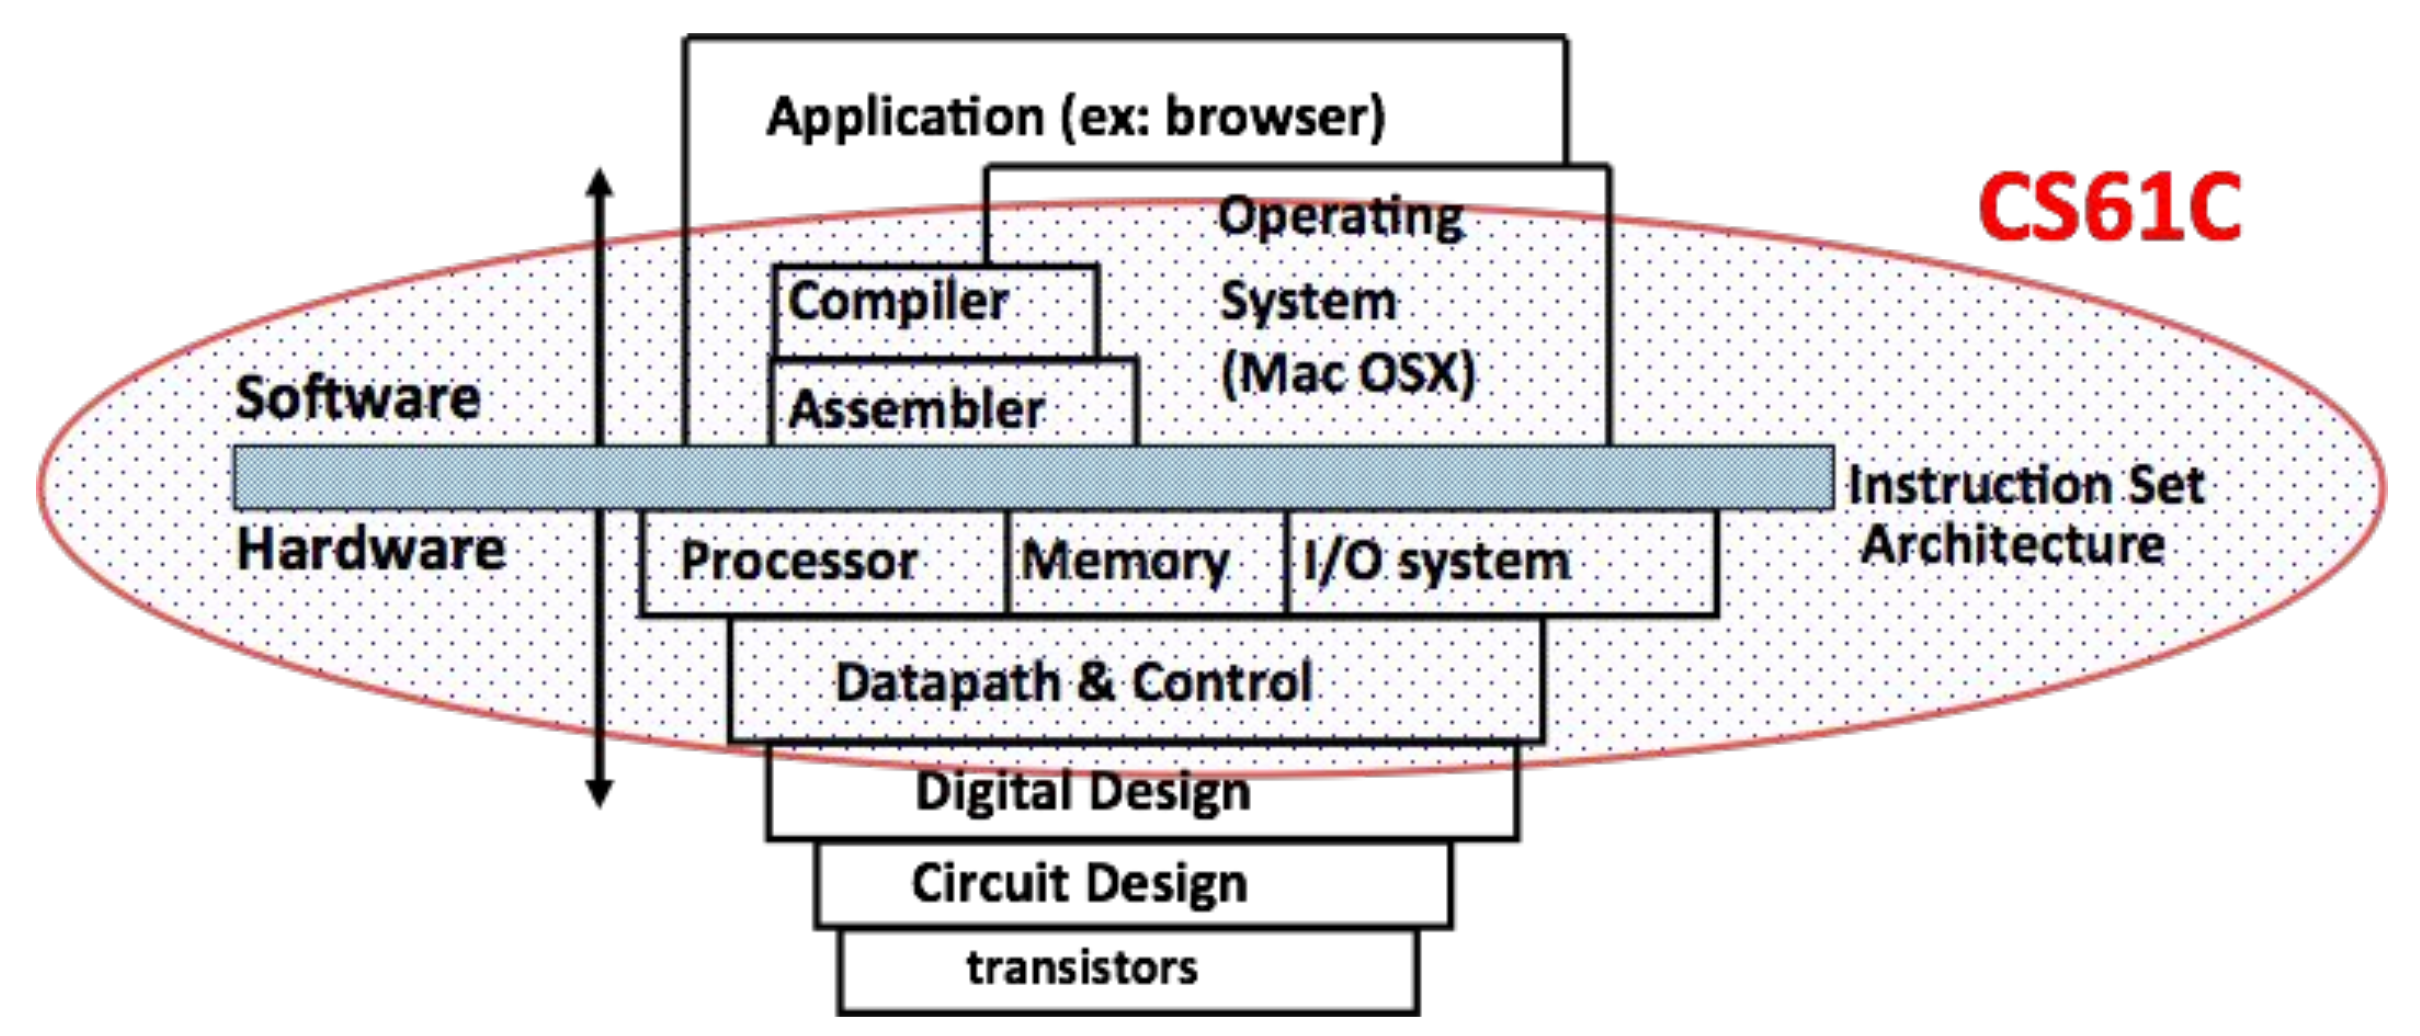
\includegraphics[width=1.4\linewidth]{hardware-software-interface}
		\caption{软硬件接口$ _{[CS-61C Berkeley]} $}
	\end{figure}
	
	% 体系结构需要易于编程/编译/链接,易于软件管理	
	
\end{frame}


\begin{frame}
	
	\frametitle{Why RISC-V}
	
	\begin{figure}
		\centering
		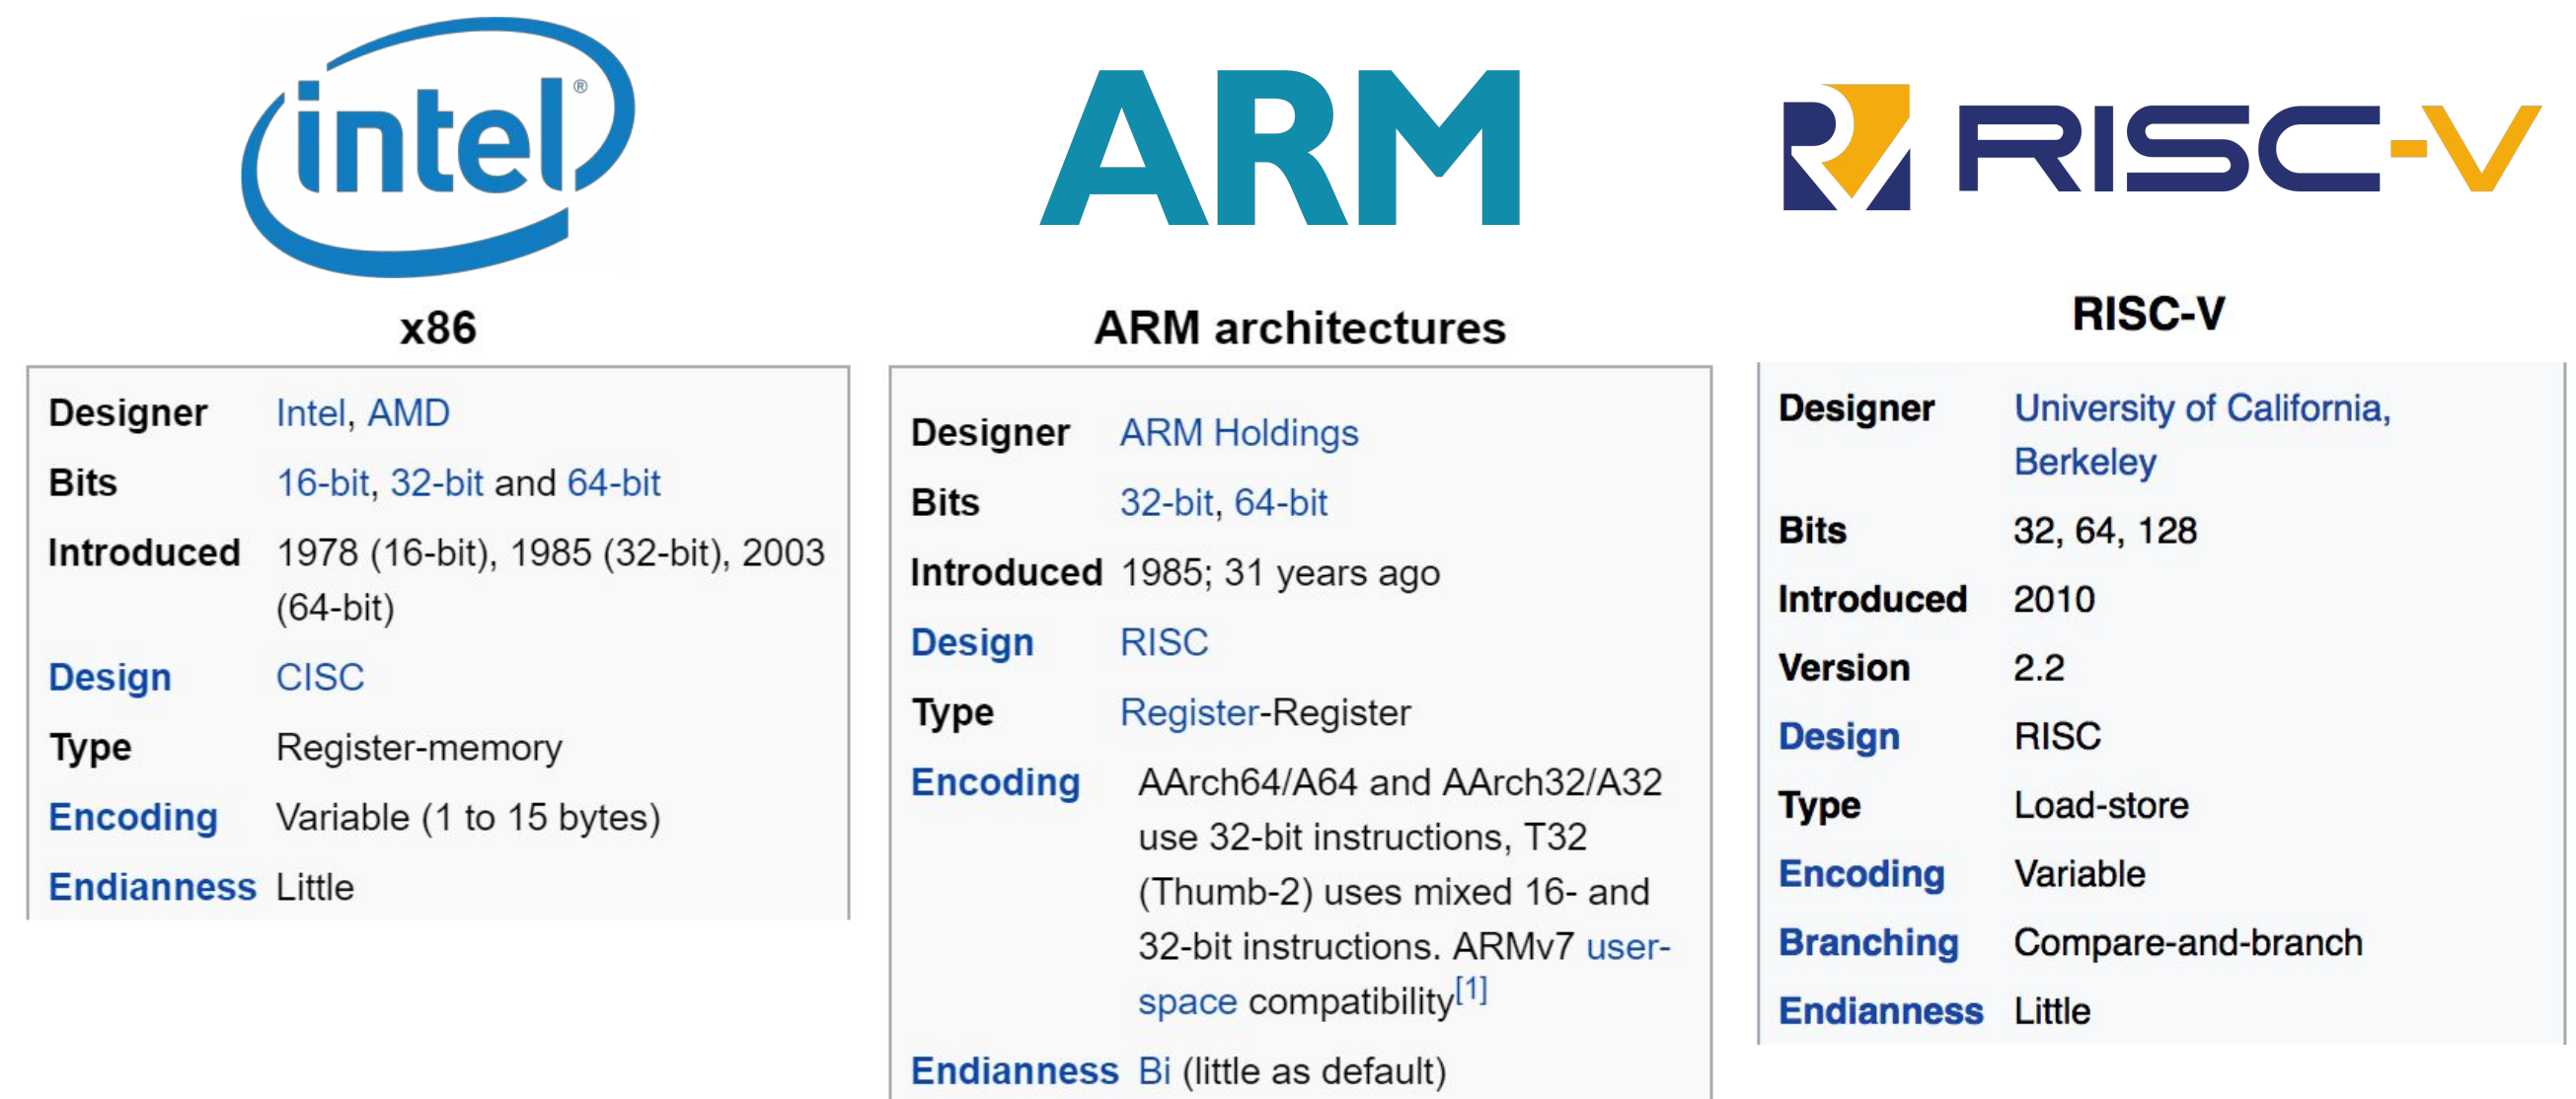
\includegraphics[width=0.75\linewidth]{mainstream-isas}
		\caption{主流的ISAs$ _{[CS-61C Berkeley]} $}
	\end{figure}
	
	\begin{figure}
		\centering
		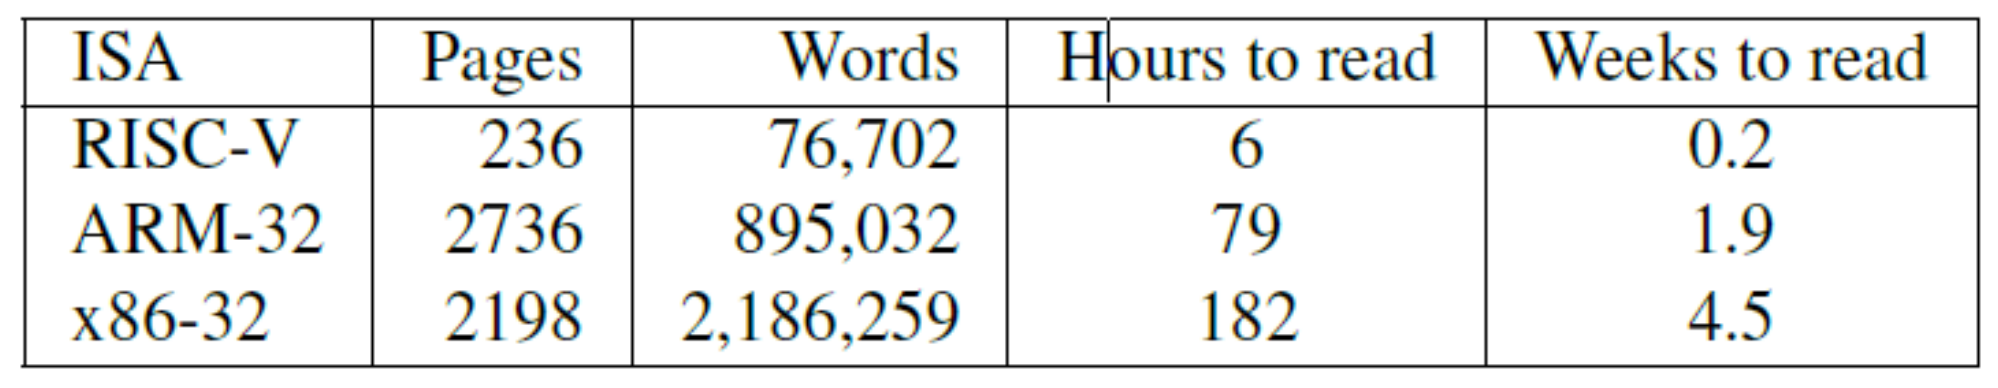
\includegraphics[width=0.65\linewidth]{x86-arm-rv-compare}
		\caption{主流CPU指令集比较$ _{[Waterman 2017]} $}
	\end{figure}
	
	
	% x86指令集自诞生以来指令数量的增长。x86在1978年诞生时有80条指令,到2015年增长了16倍	
	
	% RISC-V的不同寻常之处,除了在于它是最近诞生的和开源的以外,还在于:和几乎所
	% 有以往的ISA不同,它是模块化的。它的核心是一个名为RV32I的基础ISA,运行一个完整
	% 的软件栈。RV32I是固定的,永远不会改变。这为编译器编写者,操作系统开发人员和汇
	% 编语言程序员提供了稳定的目标。模块化来源于可选的标准扩展,根据应用程序的需要,
	% 硬件可以包含或不包含这些扩展。	
	
\end{frame}

\begin{frame}
	\frametitle{RISC-V特权架构}
	\framesubtitle{隔离}
	
	\begin{figure}
	\centering
	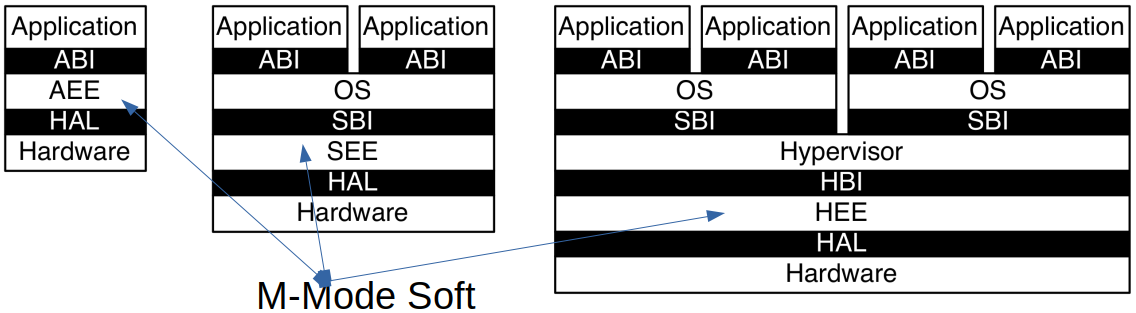
\includegraphics[width=0.9\linewidth]{rv-privil-arch}
	\caption{RISC-V特权架构}
	\end{figure}

\begin{itemize}
	
	\item 不同软件层有清晰的硬件隔离
	\item AEE: Application Execution Environment
	\item ABI: Application Bianry Interface
	\item \textbf{MODE} -- \textbf{U}: User | \textbf{S}: Supervisor | \textbf{H}: Hypervisor | \textbf{M}: Machine

\end{itemize}

\end{frame}

\begin{frame}
		\frametitle{RISC-V特权模式架构}
		\framesubtitle{隔离}
\begin{table}[h]
	\caption{RISC-V的特权模式组合}
 	\centering
 	\begin{tabular}{|c|c|l|c|l|}
 	\hline
	0 & 00 & User/Application & U \\\hline
	1 & 01 & Supervisor & S \\\hline
	2 & 10 & Hypervisor & H \\\hline
	3 & 11 & Machine & M \\\hline
   \end{tabular}

\begin{itemize}
	
	\item M, S, U  for systems running Unix-like general operating systems
	%内核模式是指RV的哪种特权模式?
\end{itemize}


\end{table}
\end{frame}




\begin{frame}
	\frametitle{RISC-V特权模式架构}
	\framesubtitle{隔离}

	\begin{itemize}
		\item 设置CSR(控制状态寄存器)实现隔离
		\begin{itemize}
			\item 防止应用程序访问设备和敏感的CPU寄存器
			\item 例如地址空间配置寄存器
		\end{itemize} 
	\end{itemize}

	\begin{itemize}
		\item 强制隔离以避免对整个系统的可用性/可靠性/安全影响
		\begin{itemize}
		\item 运行的程序通常是是隔离的单元
		\item 防止恶意程序、病毒、木马破坏或监视程序Y,扰操作系统	
			\begin{itemize}
			\item 读/写内存: mstatus/satp CSR
			\item 使用100%的CPU:mstatus/stvec CSR
			\item 更改FD:??? CSR
			% mstatus/satp/stvec CSR 页表异常处理
			\end{itemize}
		\end{itemize}
	\end{itemize}

\end{frame}



\begin{frame}{plain}
	
	\frametitle{RISC-V虚拟内存}
	
	\begin{figure}
		\centering
		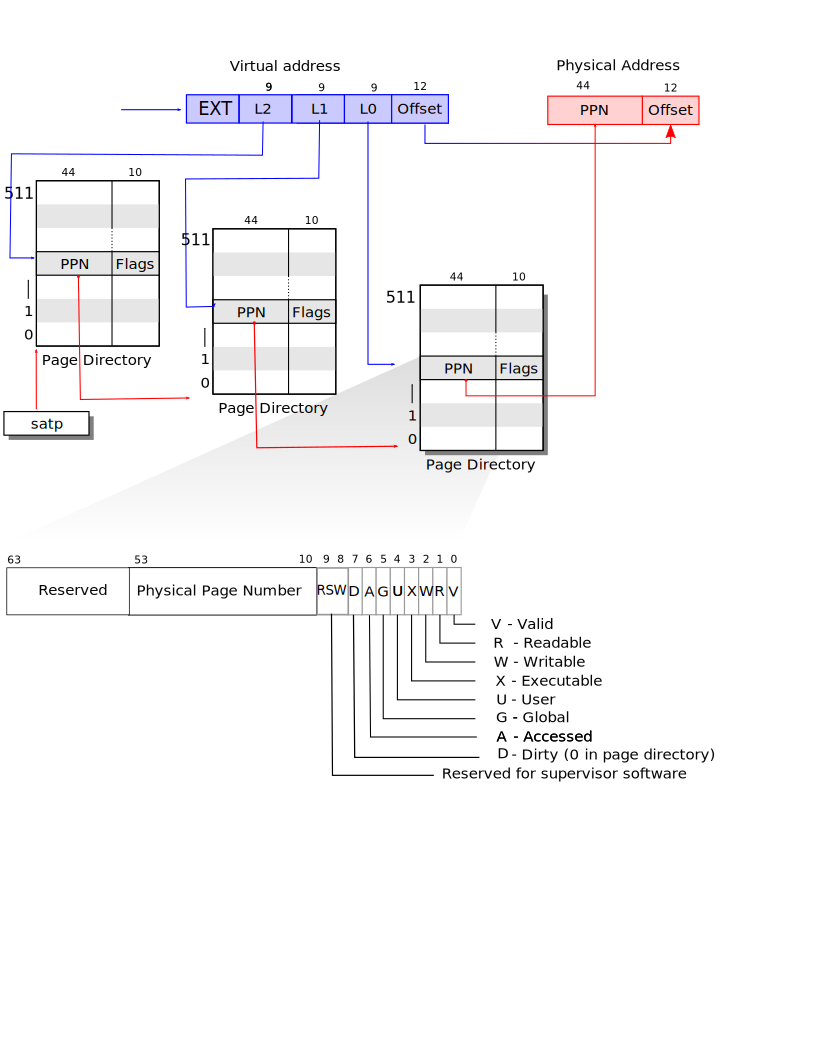
\includegraphics[width=0.65\linewidth]{riscv_pagetable}
		\caption{RISC-V虚拟内存}
	\end{figure}
	
	
\end{frame}


\begin{frame}
	\frametitle{RISC-V中断机制}
	\begin{itemize}
		\item 中断是异步发生,是来自处理器外部的I/O设备的信号的结果。
		
		
		\item Timer可以稳定定时地产生中断
		\begin{itemize}
			\item 防止应用程序死占着CPU不放,让OS kernel能得到执行权...
		\end{itemize}				
		
	\end{itemize}

	\begin{figure}
	\centering
	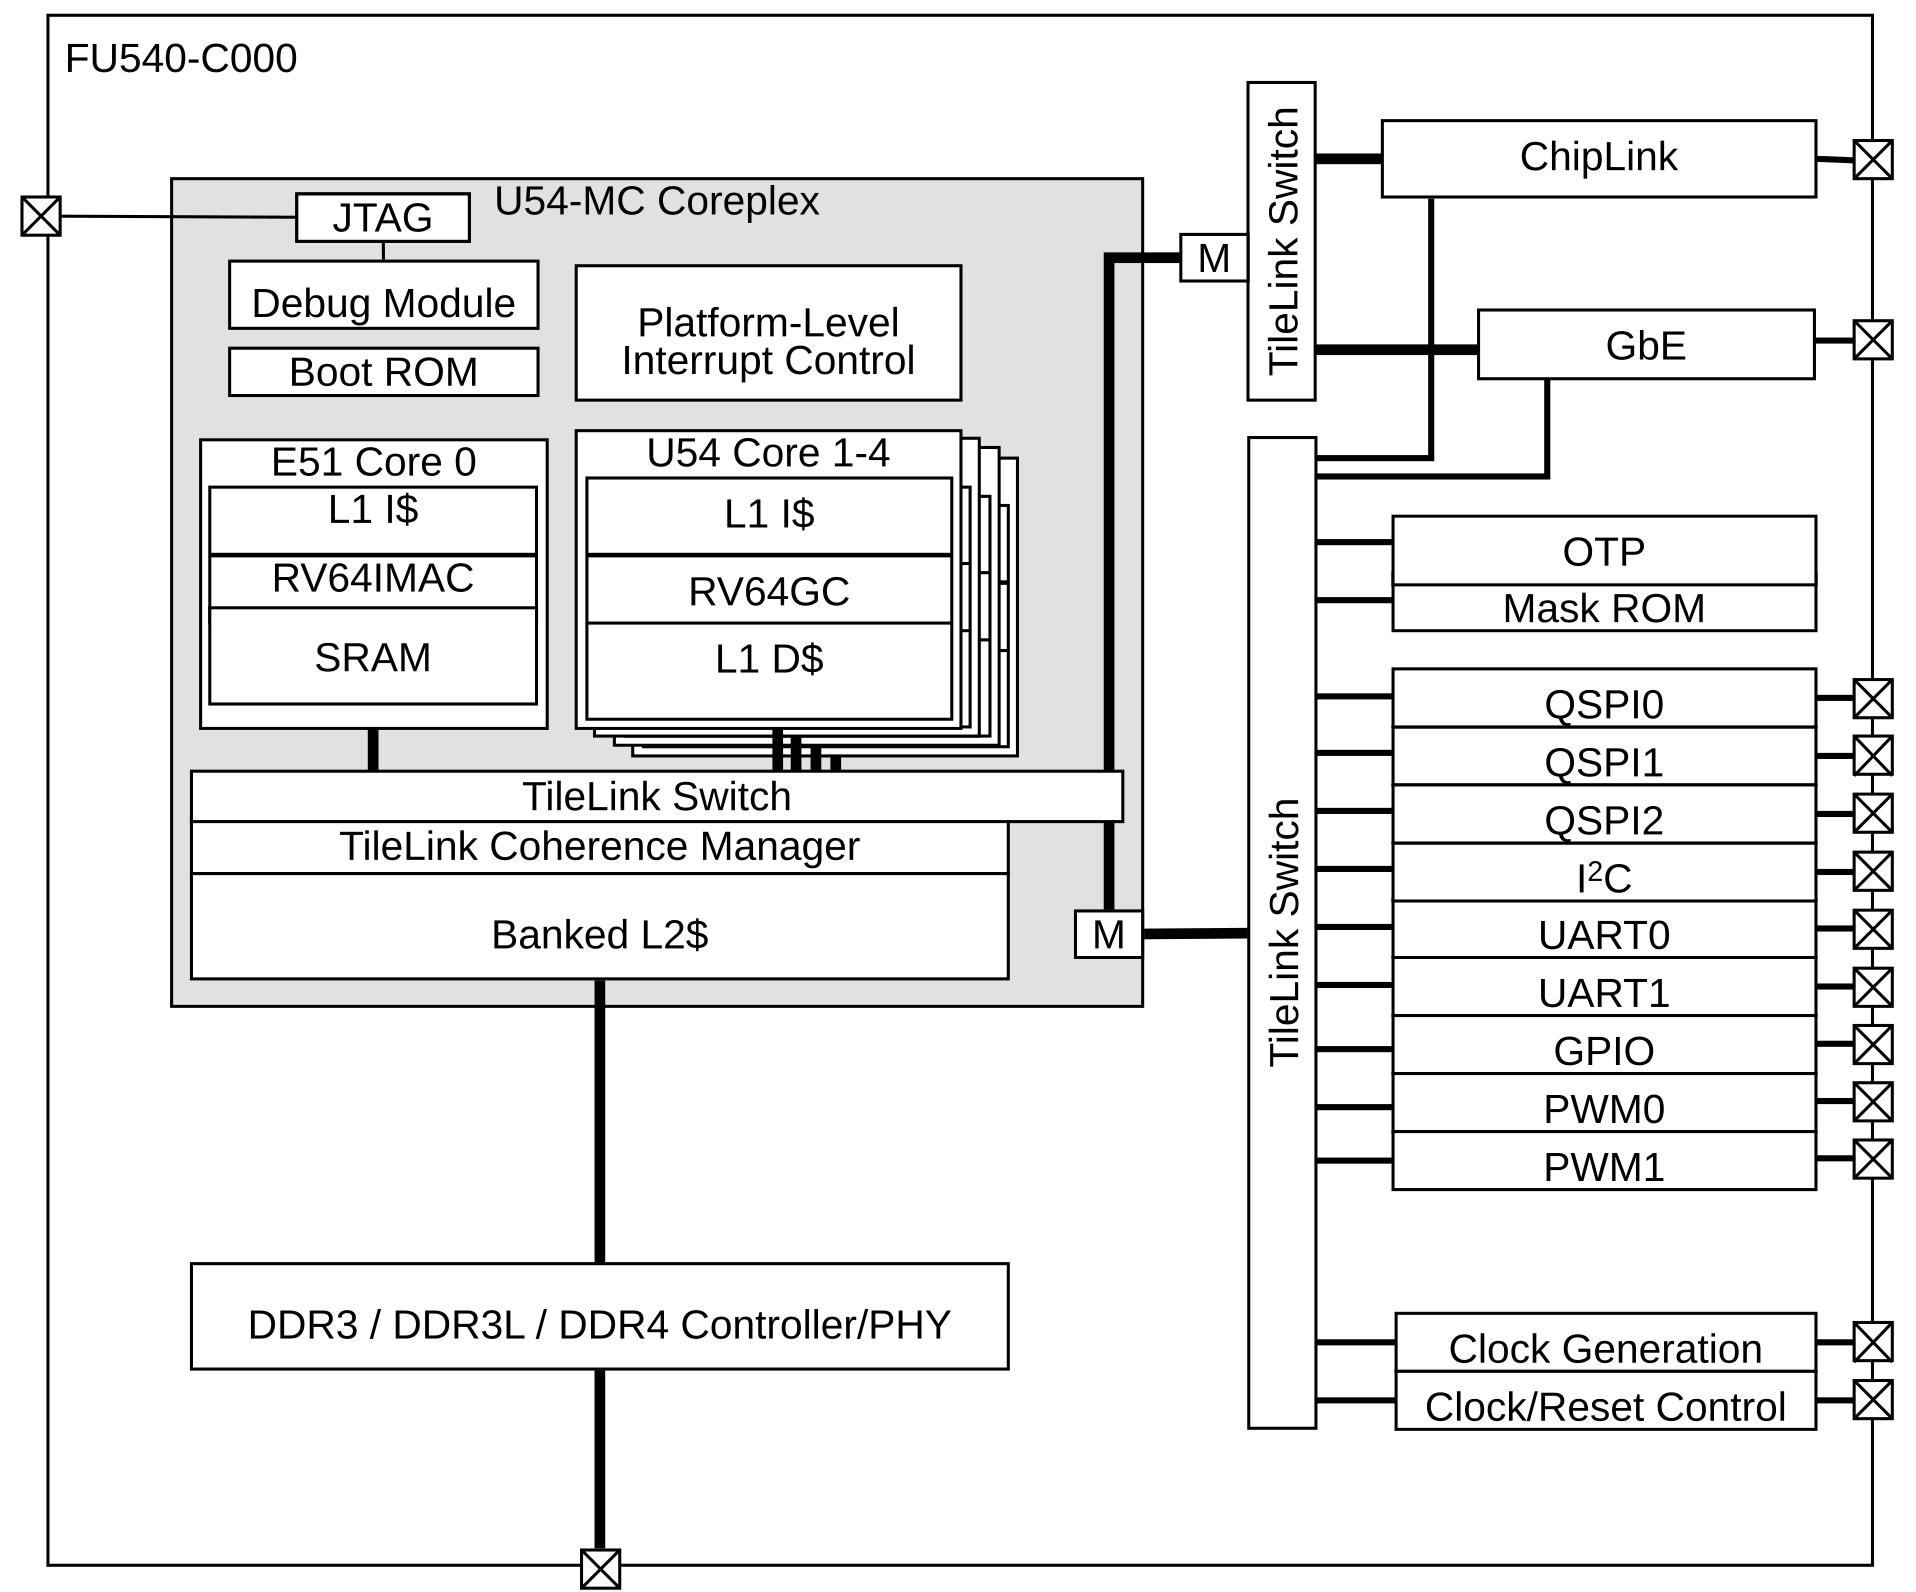
\includegraphics[width=0.65\linewidth]{fu540-top-block}
	\caption{RISC-V中断机制}
\end{figure}

\end{frame}

%----------------------------------------------------------------------------------------

\end{document}
